\section{Game References}
The art style and gameplay of \ourgame{} is influenced by many existing games, some of which are successful, some which are similar, and some which are simply inspiring. These games were played by \ourteam{} in preparation for the development of \ourgame{}. Positives and negatives about each game were discussed regarding both the style and gameplay. Different aspects from these games contributed to shaping \ourgame{} as a whole.

\begin{figure}[H]
\centering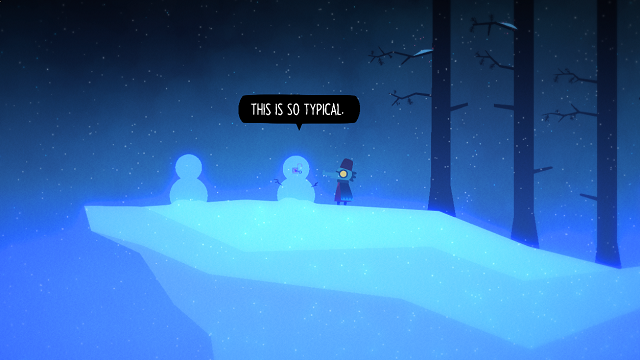
\includegraphics[width=0.7\linewidth]{images/game_references}
\end{figure}


% this fixes the weird indenting on the nested lists by moving them to a new line
\setlist[itemize]{topsep=0pt,before=\leavevmode\vspace{-1.5em}}
\setlist[description]{style=nextline}

\clearpage
\subsection{The Yawhg}
\begin{description}
\item[Description]{The Yawhg is a casual choose-your-own-adventure game for one to four players that randomizes the story during each playthrough. The players must make choices for the townsfolk about how they will spend their time as "the Yawgh" approaches, eventually deciding what they will do when it arrives.

\begin{figure}[htb]
	\centering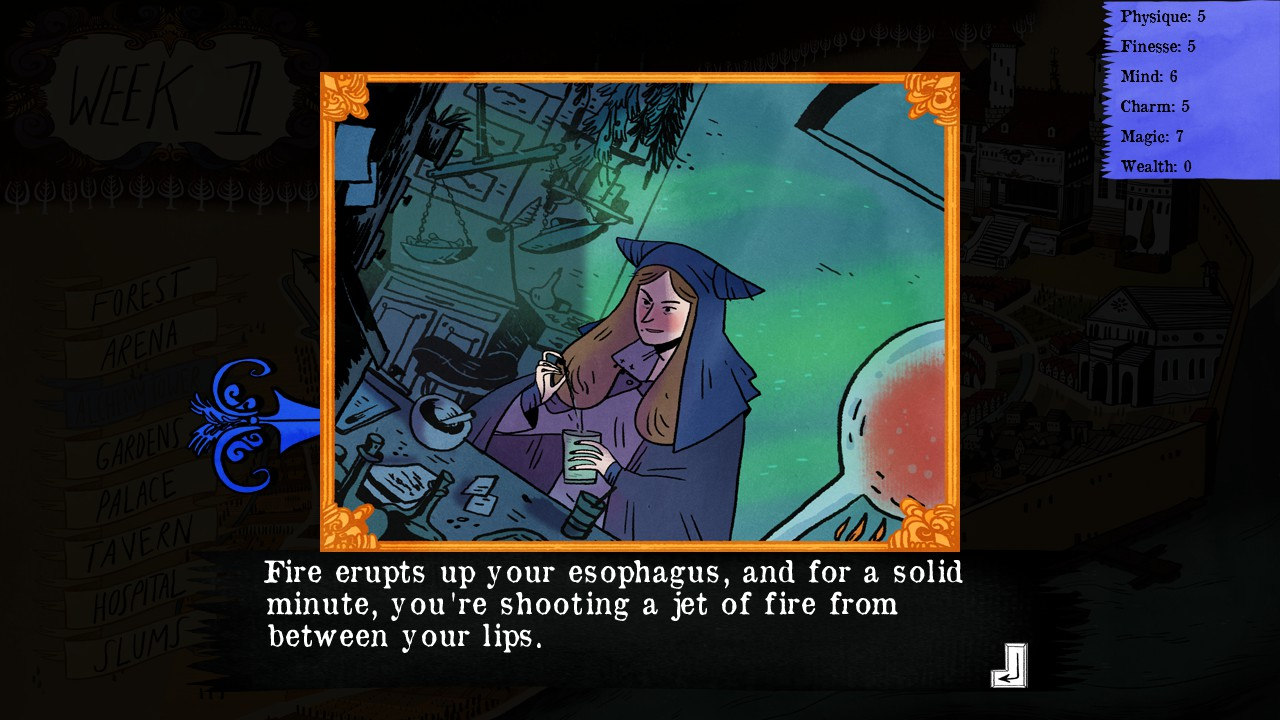
\includegraphics[width=.25\linewidth]{images/game_yawhg}
	\caption{The Yawhg - Typical result of making a choice in the game.}
	\label{fig:yawgh}
\end{figure}}
\item[Positives]{
\begin{itemize}
  \item {Almost all interactions have a net positive, even if there are negative results to immediate decisions. This allows for constant progression in the game, and puts less pressure on the players, supporting the casual atmosphere of the game.} 
  \item {The game is often humorous. In addition to making it generally more enjoyable, it makes bad results more entertaining for the player.}
  \item {Choices are typically not morally binary, making decisions more engaging and giving them more weight.}
  \item {Choices made early in the game affect random events later on. This makes players feel that their decisions have more impact, and encourages replayability as each playthrough has more potential variety.}
  \item {The game environment changes over time and with specific story events, creating the feeling of passing time and lending importance to the players' choices.}
\end{itemize}
}
\item[Negatives]{
\begin{itemize}
  \item {Some choices are presented which have a very clear "right" answer. By making outcomes too obvious, the fun of making a choice is lost.}
  \item {Large blocks of text can be boring, and they are often reused in subsequent playthroughs, significantly reducing the replayability.}
  \item {Although the game includes "good" and "bad" endings which strongly commit to a narrative, playing the game casually almost always results in neutral endings. These often have less impact and disappoint the players.}
\end{itemize}
}
\item[Take-away]{The main take-away from The Yawgh is that \ourteam{} felt that, although many of the game's aspects were interesting, the usual lack of a strong ending resulted in a feeling of dissatisfaction. As \ourgame{} is similarly focused on narrative and gives the player choices on how to progress, the variable endings must all have the ability to satisfy the player and resonate with their decisions.}
\end{description}


\clearpage
\subsection{Off-Peak}
\begin{description}
\item[Description]{Off-Peak is a 3D first person adventure game which takes place in a large train station. The player explores the secrets that the station has to offer, with the game ending as the player is eventually forced to leave. Off-Peak is a strange game full of strange characters, many of which hint at deeply involved internal lore and backstory.

\begin{figure}[htb]
	\centering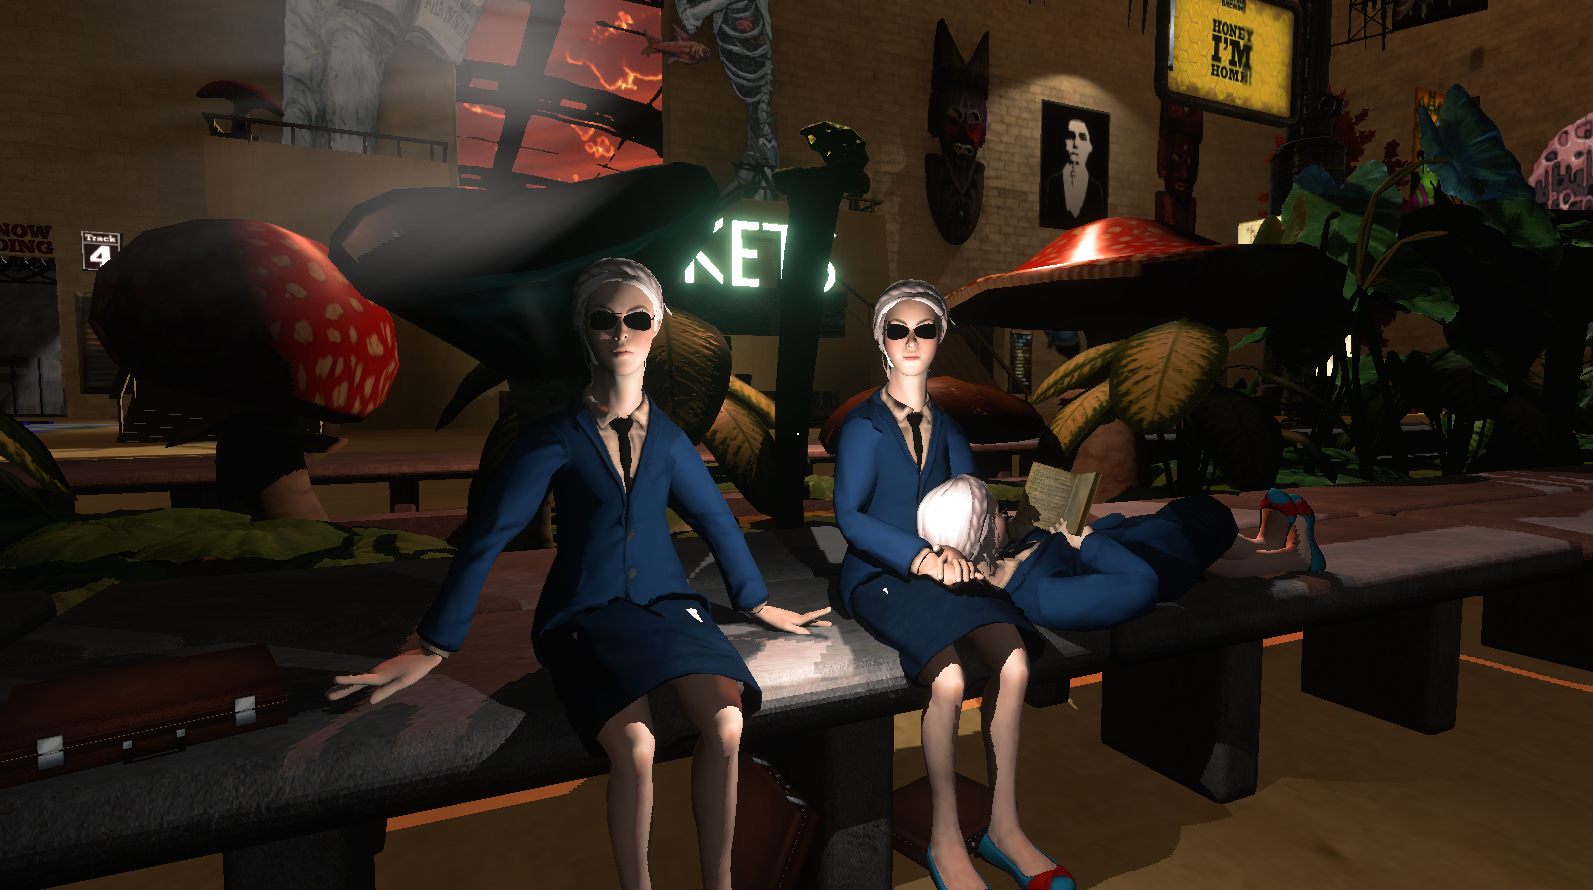
\includegraphics[width=.25\linewidth]{images/game_offpeak}
	\caption{Off-Peak - The world of Off-Peak is filled with many strange and interesting characters.}
	\label{fig:offpeak}
\end{figure}}
\item[Positives]{
\begin{itemize}
\item{The design of the game environment seemed very cohesive. The game included many details for attentive players that tie characters and world elements together.}
\item{\ourteam{} found many of the characters to be interesting.}
\end{itemize}
}
\item[Negatives]{
\begin{itemize}
\item{The game environment incorporates many visual references and homages, but these often felt hollow as the references are not well integrated and seem to simply be a nod to more successful works.}
\item{Fast readers find it annoying that the player cannot manually advance incidental dialogue and get bored waiting for it to progress automatically.}
\item{Incidental conversations will loop without delay. This makes it unclear when they actually start/end.}
\item{The integration of dialogue text into the 3D environment often makes it difficult to read and causes eye strain.}
\item{The game constantly alludes to a larger backstory, but never elaborates or delivers on this foreshadowing.}
\item{Many characters don't react or barely react to the player's actions. This makes the many of the interactions feel pointless.}
\item{The player can turn away from dialog accidentally and miss interesting information.}
\item{Only certain characters were capable of interaction. This was disappointing, as some of the non-interactive characters seemed more interesting than the interactive ones.}
\end{itemize}
}
\item[Take-away]{Although \ourteam{} found that Off-Peak was an interesting experience with many parallels to \ourgame{} (specifically, the plot revolves around the train station's mysterious patron and the player spends much of their time uncovering mysteries), their were many missteps that \ourteam{} hopes to avoid. In particular, the dialogue system in \ourgame{} will have to present text and accompanying audio in such a way that players cannot mistakenly miss.

Additionally, one of Off-Peak's greatest mistakes in the eyes of \ourteam{} is that the amount of time spent with characters seemed inversely proportional to how interesting they were. A lot of time needs to be spent polishing the game's main plot in order to keep it interesting, and there needs to be plenty of side content to keep players entertained should they find the plot boring.}
\end{description}



\clearpage
\subsection{Slave of God}
\begin{description}
\item[Description]{Slave of God is a first-person narrative game about meeting someone at a nightclub. The story is revealed to the player through a unique mix of level design and visuals. The game was created by independent developer Stephen Lavelle.

\begin{figure}[htb]
	\centering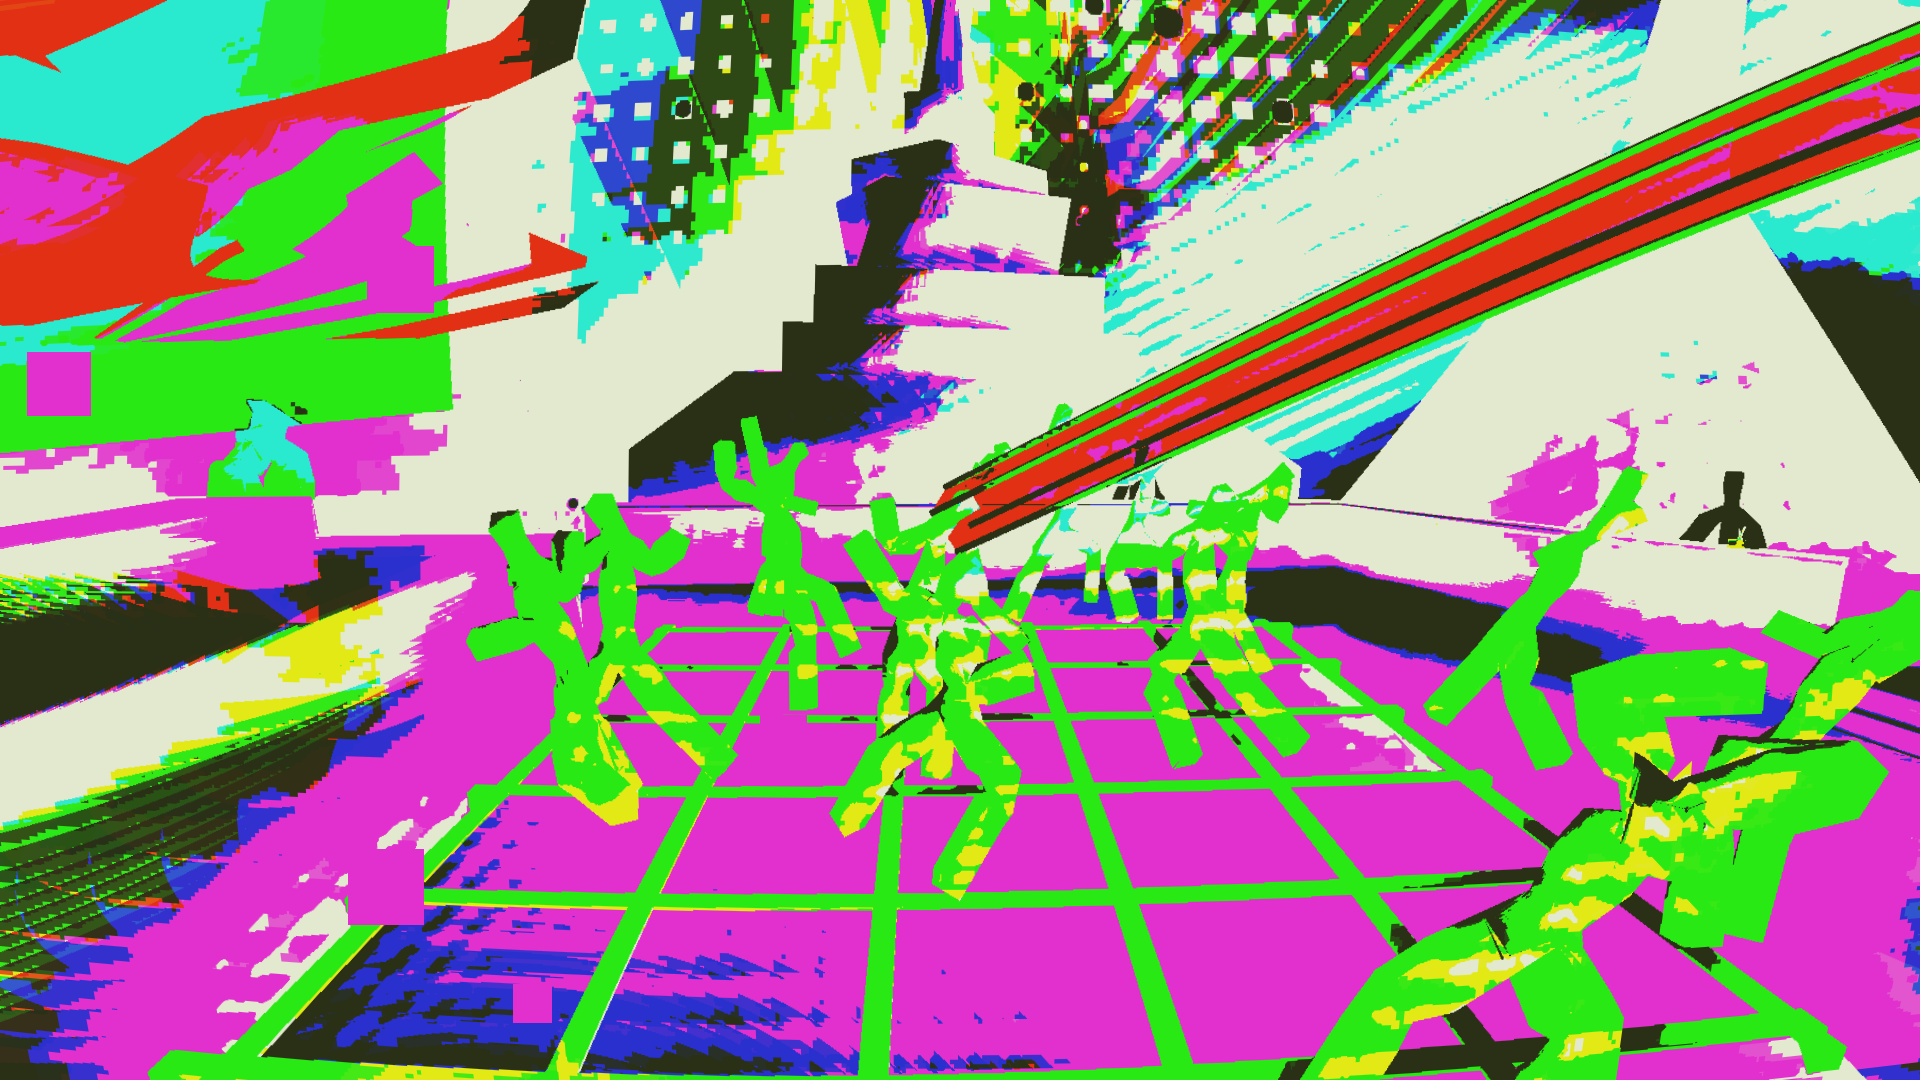
\includegraphics[width=.25\linewidth]{images/slave}
	\caption{Slave of God - A view of the dancefloor. The characters are crude 3D stick figures. The game world flashes and changes colours with the music.}
\end{figure}}
\item[Positives]{
\begin{itemize}
\item{The game very accurately recreated the experience of attending a nightclub, through audio-visual distortions and some interesting custom shaders.}
\item{Important elements of the story are communicated through the environment. For example, the lack of a women's washroom suggests that the club is for men only.}
\end{itemize}
}
\item[Negatives]{
\begin{itemize}
\item{The game is purposefully confusing to process and difficult to navigate, but some members of \ourteam{} found it frustrating to figure out how to progress through the environment and discover new parts of the narrative.}
\end{itemize}
}
\item[Take-away]{\ourteam{} enjoyed the way the audio and visuals of Slave of God created a convincing nightclub environment. However, the visuals and level design were confusing and not very accessible. The mansion layout in \ourgame{} should have a lot of space to navigate, and the visuals should not overly obscure the systems or environments.

The environmental story was a key part of Slave of God and will be for \ourgame{} as well. The design for the mansion should take into consideration the plot and characters, and should include items the player can discover to learn more about Omar Clean and his motivations.}
\end{description}




\clearpage
\subsection{Psychonauts}
\begin{description}
\item[Description]{Psychonauts is a third person action game where players take control of a young psychic attending a secret camp for gifted children, learning how to use their special powers.

\begin{figure}[htb]
	\centering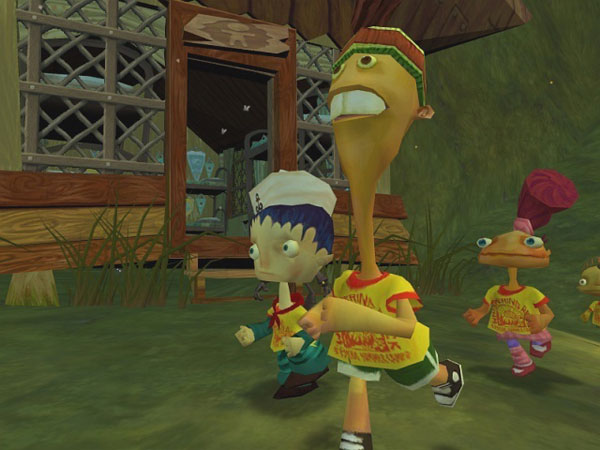
\includegraphics[width=.25\linewidth]{images/game_psychonauts}
	\caption{Psychonauts - An example of diverse characters found within the game.}
\end{figure}}
\item[Positives]{
\begin{itemize}
\item{The game includes many interesting characters with memorable designs.}
\item{The game varies greatly as the player progresses through different levels, each with their own themes.}
\item{Visual styles, though varied, fit together to create a complex and cohesive world that incorporates the works of many different artists.}
\item{Dialogue throughout the game is funny and keeps the audience engaged, even when exploring side plots.}
\end{itemize}
}
\item[Negatives]{
\begin{itemize}
\item{A massive difficulty spike near the end of the game prevented many from completing the game.}
\item{There is a huge amount of content in between main story elements that can be easily missed as the game heavily directs the player through the main story-line.}
\end{itemize}
}
\item[Take-away]{The art of Psychonauts is visually strange, but remains appealing despite impossibly exaggerated character proportions. It inspired the procedural character generation system in which characters of wildly varying shapes, sizes, and proportions can be created without fear of artistic dissonance. Psychonauts is also an example of an early game which favoured comedic writing over finely tuned gameplay. Its cult success proves that there are many players that prioritize humour and well-written characters over mechanical perfection. }
\end{description}



\clearpage
\subsection{Planetarium}
\begin{description}
\item[Description]{Planetarium is a procedurally generated interactive experience in which the player can explore and terraform planets. Each planet has an ideal temperature, and the player will be rewarded with additional flavour text describing life on the planet.

\begin{figure}[htb]
	\centering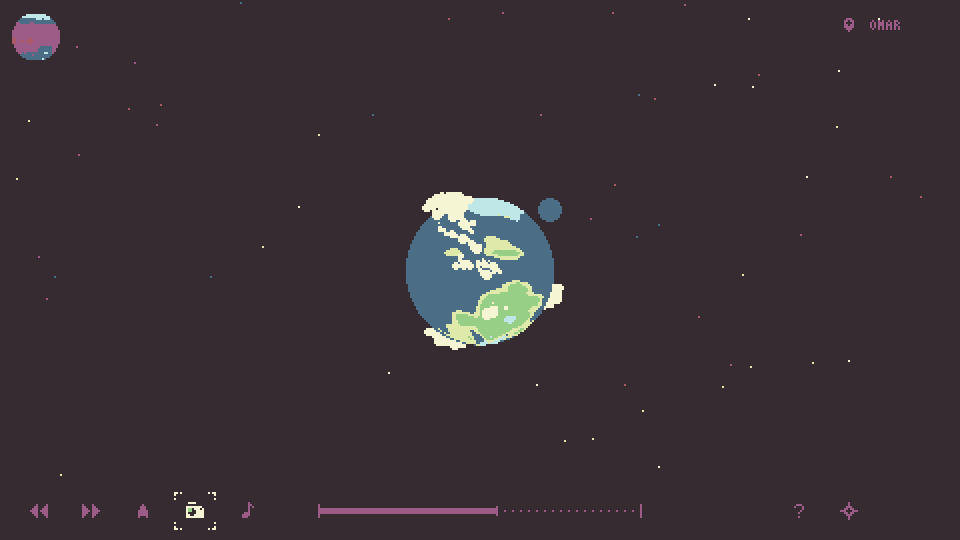
\includegraphics[width=.25\linewidth]{images/game_planetarium}
	\caption{Planetarium - Planet OMAR, one of the virtually infinite discoverable planets in Planetarium.}
	\label{fig:planetarium}
\end{figure}}
\item[Positives]{
\begin{itemize}
\item{Appealing visual style.}
\item{As the game is highly focused on visual aesthetics, the inclusion of a dedicated screenshot button was welcome.}
\item{The use of deterministic procedural generation encourages propagation through word-of-mouth, as players can share interesting planet seeds with others.}
\end{itemize}
}
\item[Negatives]{
\begin{itemize}
\item{The interactivity is very limited and poorly explained.}
\item{The only explicit reward for interaction is a small amount of flavour text.}
\end{itemize}
}
\item[Take-away]{As \ourgame{} makes heavy use of procedural generation, ensuring that the random elements are all deterministic would allow \ourteam{} to let players share seeds for specific parties.}
\end{description}


\clearpage
\subsection{Doom}
\begin{description}
\item[Description]{Doom is a classic FPS and one of the most influential games of all time. The player takes the role of a space marine fighting demons, all taking place in one of the earliest 3D engines in the history of game design.

\begin{figure}[htb]
	\centering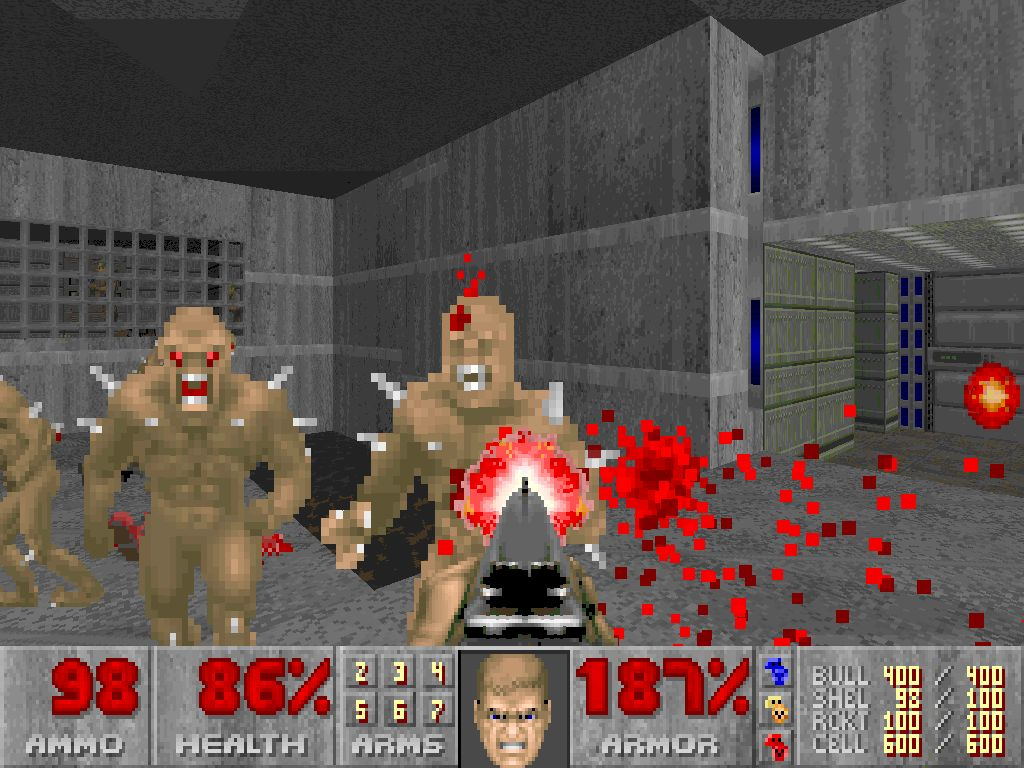
\includegraphics[width=.25\linewidth]{images/game_doom}
	\caption{Doom - Although it made use of a 3D environment, characters in Doom were all represented as 2D billboards.}
	\label{fig:doom}
\end{figure}}
\item[Positives]{
\begin{itemize}
\item{Billboarded characters placed in a 3D environment did not seem to interfere player's perception of the game world.}
\end{itemize}
}
\item[Negatives]{
\begin{itemize}
\item{The level of difficulty is a major drawback for some players. Even on the easiest setting, some players cannot progress through the game and give up.}
\item{The lack of variation in the level design makes navigation annoying.}
\end{itemize}
}
\item[Take-away]{By playing Doom, \ourteam{} gained assurance in their decision to render 2D characters in a 3D environment due to the fact that it did not seem to distract players. \ourteam{} also took note that layouts that are overly complex can make gameplay frustrating.}
\end{description}



\clearpage
\subsection{Little Party}
\begin{description}
\item[Description]{Little Party is a game in which the player takes on the role of a middle-aged widowed housewife, chaperoning an art jam for her twenty-something daughter and her friends. Throughout the game, the player interacts with their daughter and guests and performs menial tasks as the mother goes about with her night. 

\begin{figure}[htb]
	\centering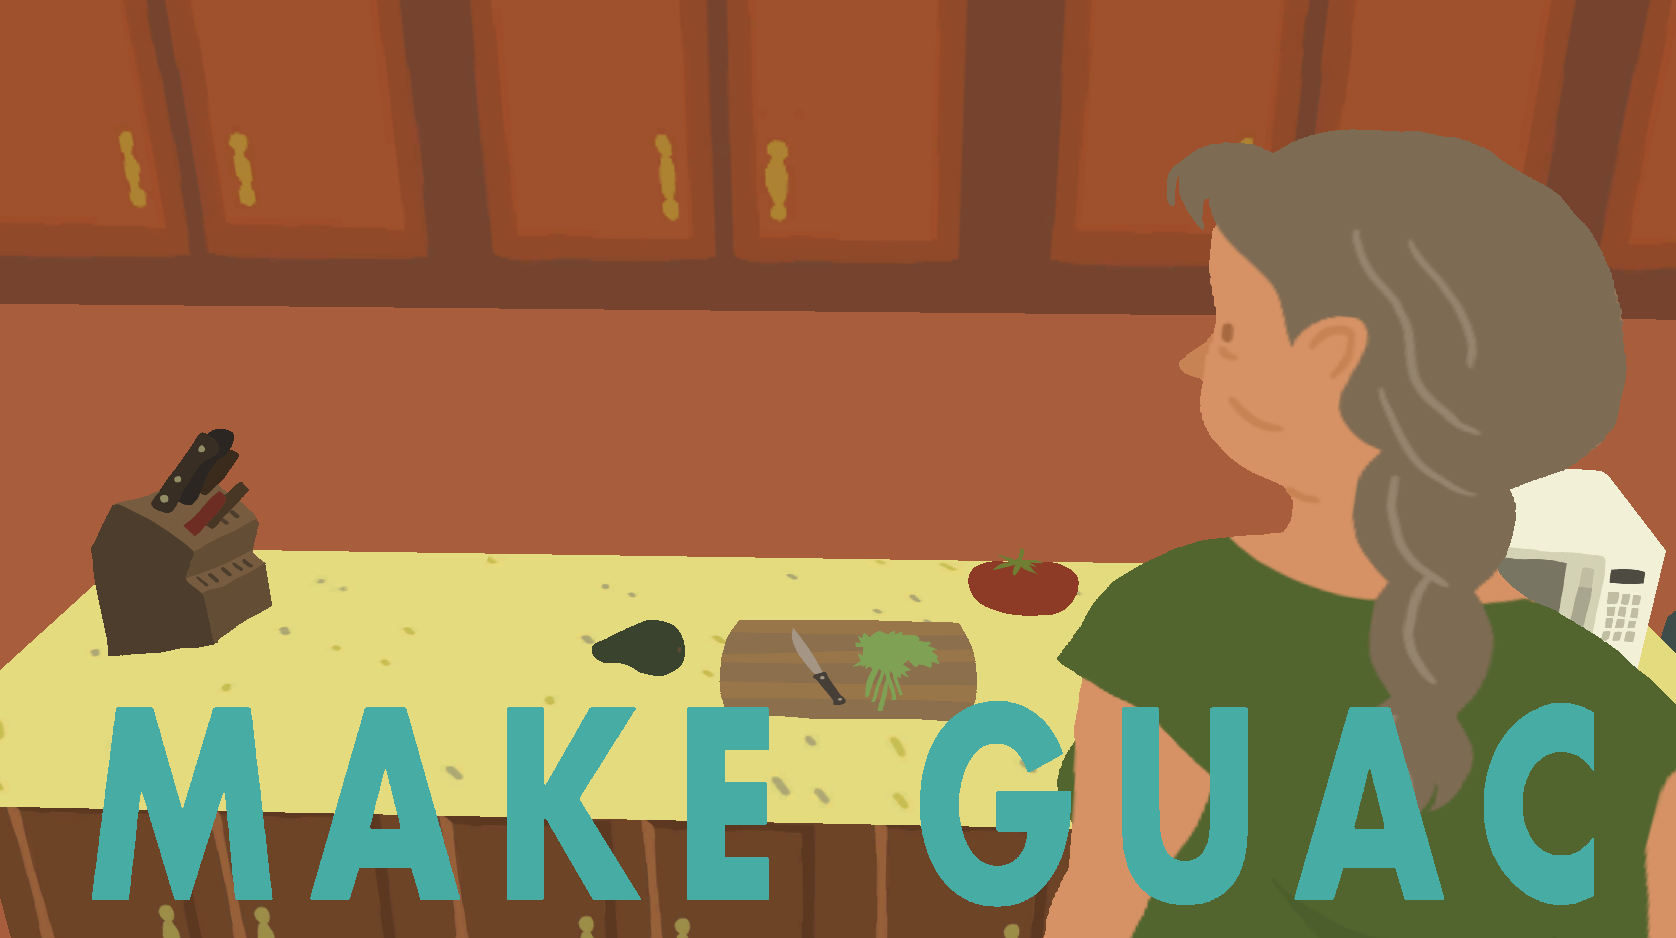
\includegraphics[width=.25\linewidth]{images/game_little_party}
	\caption{Little Party - Exciting mom on guac action.}
	\label{fig:little_party}
\end{figure}}
\item[Positives]{
\begin{itemize}
\item{The character transition method in which characters simply teleport while the player cannot see them.}
\item{Short and simple character animations helped bring life to characters.}
\item{The use of positional audio made the experience more immersive.}
\end{itemize}
}
\item[Negatives]{
\begin{itemize}
\item{The camera perspective makes navigation very difficult and detracts from the visual experience.}
\item{Some members of \ourteam{} found the experience too boring to play for more than a few minutes.}
\item{The conversation dialogue hid the characters/environment, making it feel cold and impersonal.}
\item{Interactive elements weren't effectively differentiated from the rest of the environment.}
\item{The player could only interact with key plot items; The environment would have felt more immersive if the player was able to interact with some non-essential items as well.}
\end{itemize}
}
\item[Take-away]{The game effectively mixed 2D and 3D assets to create the game world. However, attempting to represent a small, cramped party environment while including the player character in a third-person camera was a poor decision, which supports \ourteam{}'s decision to put make the camera a first-person perspective in \ourgame{}.}
\end{description}



\clearpage
\subsection{Crypt of the NecroDancer}
\begin{description}
\item[Description]{Crypt of the NecroDancer is a hybrid of games in the rogue-like dungeon crawler genre and fast-paced rhythm games like Dance Dance Revolution. The player must progress through a fairly standard gameplay loop in which they defeat enemies, find items, and work their way downwards to the final boss battle, all while under the pressure of keeping the beat.

\begin{figure}[htb]
	\centering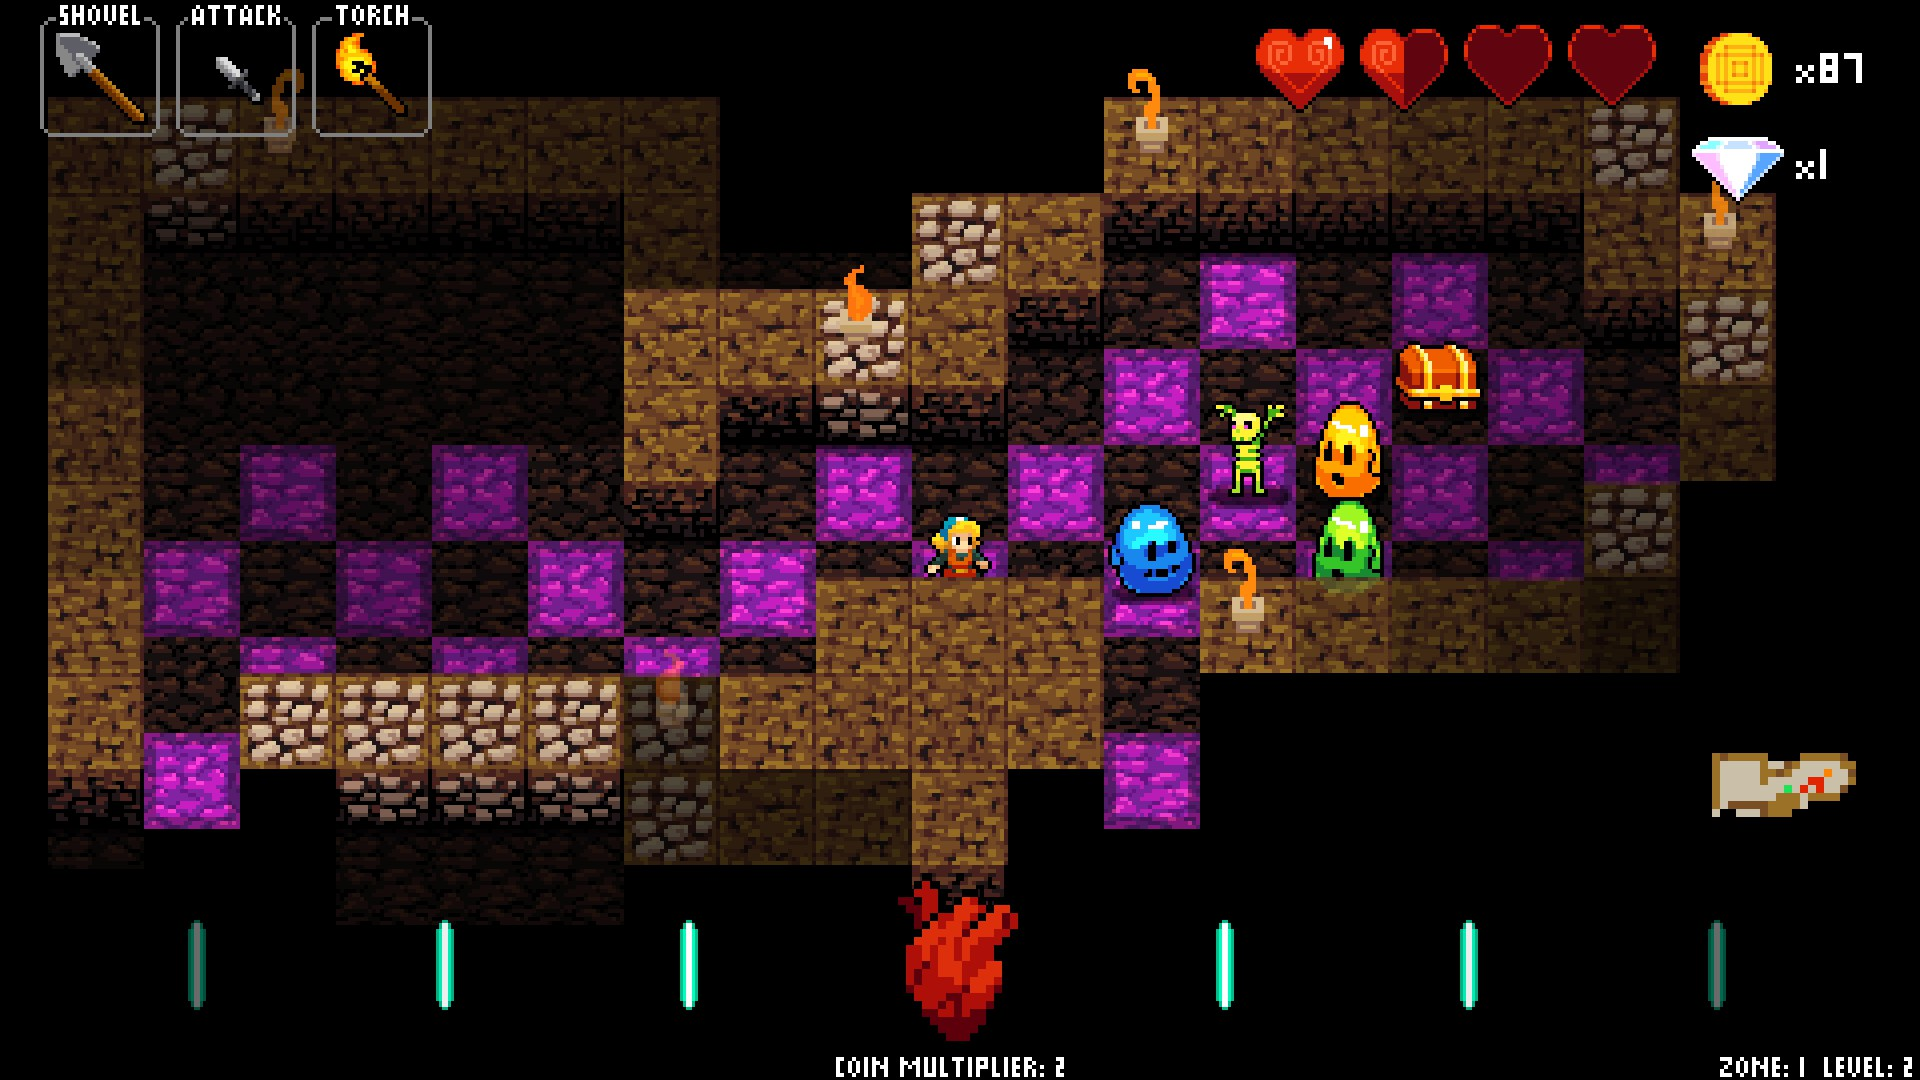
\includegraphics[width=.25\linewidth]{images/game_cotn}
	\caption{Crypt of the NecroDancer - The frantic pace of Crypt of the NecroDancer complements its disco style.}
	\label{fig:crypt_of_the_necrodancer}
\end{figure}}
\item[Positives]{
\begin{itemize}
\item{As a rogue-like, the game has a steep learning curve, but the game mechanics encourage player learning rather than mechanical progression in order to offset this.}
\item{The audio-visuals for the game are highly polished.}
\item{Positional audio helps the player quickly locate specific threats or benefits even when they are off-screen.}
\item{The player is able to unlock more powerful items and hints on how to defeat powerful enemies using diamonds acquired during their runs. This feature allows players of a lower skill level to feel as if they are making more progress.}
\end{itemize}
}
\item[Negatives]{
\begin{itemize}
\item{The local multiplayer mode felt like it was tacked on, and was usually too cramped and confusing for players to progress and survive effectively.}
\end{itemize}
}
\item[Take-away]{Overall, \ourteam{} was impressed by Crypt of the NecroDancer. One of the main elements that struck the team was the way the story is revealed to the player by having them complete multiple playthroughs under different circumstances. The planned progression in \ourgame{} is going to be similar to this.

This game also highlighted the problem with under-developed features: the local multiplayer mode did not add much to the experience because it felt poorly implemented, and if anything, made it feel less polished as a whole.}
\end{description}




\clearpage
\subsection{Crypt Worlds}
\begin{description}
\item[Description]{Crypt Worlds is an eccentric first person exploration/adventure game. The setting is inspired by early FPS games like Doom, and mixes the retro visual style with cyberpunk and Lovecraftian elements. The gameplay is unconventional, and revolves around a urine-based resource system.

\begin{figure}[htb]
	\centering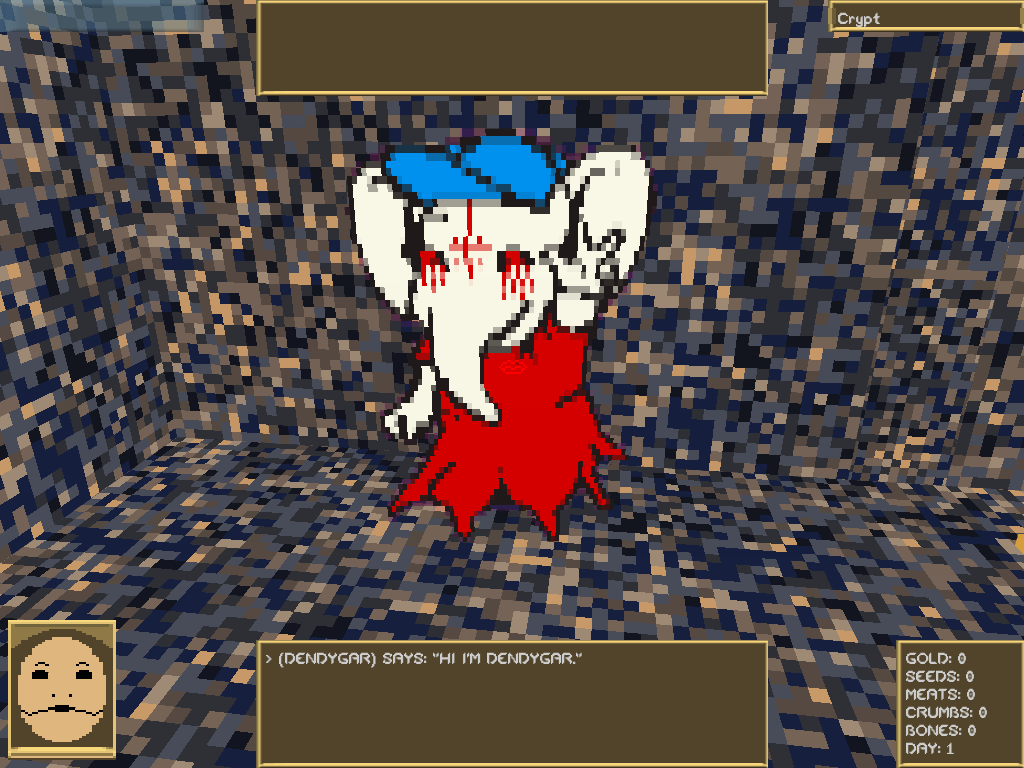
\includegraphics[width=.25\linewidth]{images/game_crypt_worlds}
	\caption{Crypt Worlds - Its a weird game.}
	\label{fig:crypt_worlds}
\end{figure}}

\item[Positives]{
\begin{itemize}
\item{The game effectively mixes 3D and 2D billboards in order to create the game world and its inhabitants.}
\item{The game's cursor updates to reflect the context-sensitive action which the player will perform. This is a very effective visual shorthand.}
\end{itemize}
}
\item[Negatives]{
\begin{itemize}
\item{The gameplay involved a lot of backtracking. This was particularly annoying because the player's speed is fixed at a slow crawl for most of the game.}
\item{The audio wasn't normalized, leading to sound effects which were too quiet mixed with some which were too loud. Similarly, the positional audio drop-off was not fine-tuned, and often caused sounds to suddenly fade in or out based on player position.}
\item{The player is penalized for experimenting with resources even though this is crucial to progression within the game. Upgrades were available that made resource expenditure less of a concern, but they are only made available towards the end of the game, after most of the resource-heavy puzzles had been solved.}
\item{The escape key quit the game entirely instead of opening a menu, as would typically be expected.}
\item{The platforming puzzles, although fairly simple, could be very difficult to complete due to the inaccuracy and unreliability of the controls.}
\end{itemize}
}
\item[Take-away]{As \ourgame{} is a game which similarly makes use of a 3D environment with 2D characters, the visual style of Crypt Worlds can be used as a good reference in terms of integrating the two mediums.

Another element of Crypt Worlds that \ourteam{} learned from is the implementation of platforming. Attempting to complete jumping puzzles from first person is typically frustrating and requires very fine-tuned physics. Although players of \ourgame{} will be given the ability to jump, this will not be used to restrict progress in order to avoid these issues of frustration.}
\end{description}



\clearpage
\subsection{Night In The Woods: Lost Constellation}
\begin{description}
\item[Description]{Lost Constellation is a 2D exploration game which includes a spooky atmosphere, story elements, and fun mini-games. It is a promotional game made in preparation for the release of Night In The Woods.

\begin{figure}[htb]
	\centering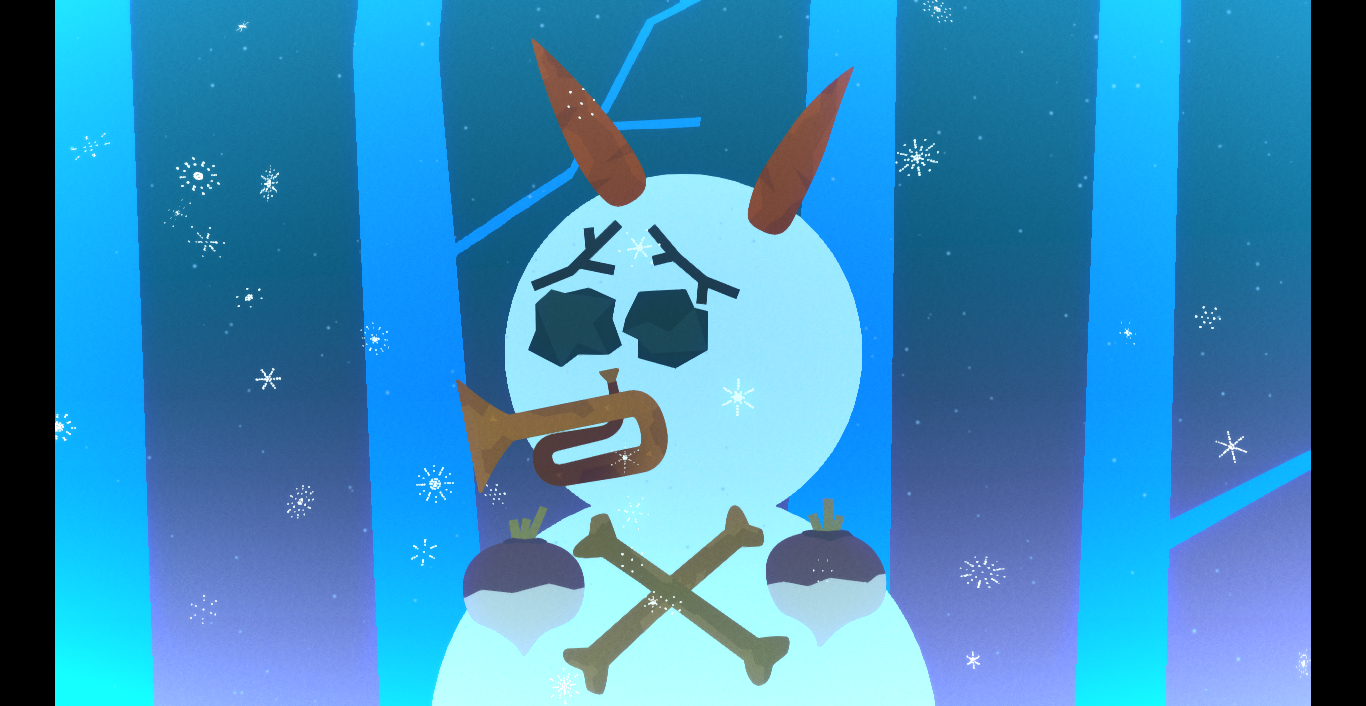
\includegraphics[width=.25\linewidth]{images/game_nitw}
	\caption{Night In The Woods: Lost Constellation - A player-made snowman, built using the components provided ingame.}
	\label{fig:nitw}
\end{figure}}

\item[Positives]{
\begin{itemize}
\item{The game has great character and art design.}
\item{One of the mini-games is particularly interesting: players are given a few unique key items, basic components, and are tasked with creating a snowman, which comes to life. Only the key items actually effect the game's progression, but providing extra elements and the freedom to place them however the player chooses makes the resulting character feel more personal.}
\item{The interface for dialogue is highly polished and shows your character's choices in a speech bubble one at a time with the option to switch. This is a much more visually pleasing method of displaying dialogue options than most games offer.}
\item{The game has a very nice loading screen.}
\item{Unlike some of the other games used as reference, most of the team found Lost Constellation's writing to be genuinely interesting. The developers clearly had specific themes they wished to communicate, and characters were more fleshed out and they played more into the world's backstory.}
\item{Very simple controls.}
\item{Puzzles had multiple solutions, and some items would produce a result but not actually progress the story. This gave the player a stronger sense of exploration and let them experiment with the items they were given.}
\end{itemize}
}
\item[Negatives]{
\begin{itemize}
\item{Many of the puzzles in Lost Constellation were revealed after the solutions to the puzzle had already been found. This was a serious misstep in design, as some players were able to intuit that they were sequence-breaking, and players which did not realize this were usually just confused by the found items.}
\item{Some of the puzzles were too obtuse for players to solve (although there was a built-in hint system to help them in case this happened).}
\item{There was no way to move the player character faster.}
\end{itemize}
}
\item[Take-away]{As \ourgame{} makes heavy use of dialogue, a sophisticated UI for presenting this dialogue will be necessary. The representation of choice in Lost Constellation greatly inspired \ourteam{}'s approach to designing the dialogue and interaction UI.}
\end{description}



\clearpage
\subsubsection{The Binding of Isaac: Rebirth}
\begin{description}
\item[Description]{The Binding of Isaac is a 2D bullet-hell, rogue-like, dungeon crawler full of Biblical references and vulgar content. The game is very difficult, and uses procedural generation to make every playthrough unique.

\begin{figure}[htb]
	\centering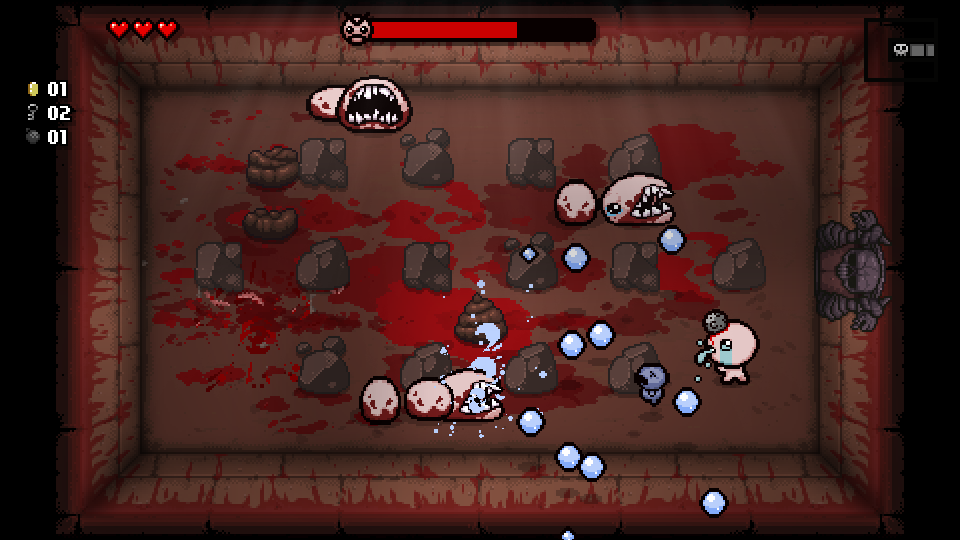
\includegraphics[width=.25\linewidth]{images/game_isaac}
	\caption{The Binding of Isaac: Rebirth - Isaac fights a boss, aided by a ghostly fetus and a meteor implanted in his skull.}
	\label{fig:binding_of_isaac}
\end{figure}}
\item[Positives]{
\begin{itemize}
\item{Almost every special type of room is visually marked on the map and/or in-game such that experienced players can quickly recognize and them and plan their playthrough accordingly. Similarly certain secrets, such as rocks which contain items, are visually differentiated from their standard counterparts.}
\item{As the player progresses through a run, their character's appearance changes to reflect the items that have been picked up. This makes each run feel more unique or personal.}
\item{The game implements a version of the rogue-like "potion trope", wherein there are a set number of pill colours and pill effects, but the mapping between the two is randomized with each playthrough.}
\item{The game greatly increases the replayability by doling out the game's mechanics and story incrementally. In order to unlock all of the content, the player must complete dozens of increasingly difficult runs.}
\end{itemize}
}
\item[Negatives]{
\begin{itemize}
\item{Although the game is procedurally generated, many of the rooms feel "cut-and-paste", as they are often just randomly selected from a set of pre-made room/enemy configurations.}
\end{itemize}
}
\item[Take-away]{One of the most effective mechanics of encouraging continued play is to reward the player with power-ups and resources within the game. This is very simple in statistic-based gameplay, such as Binding of Isaac's combat upgrades and modifiers. The incorporation of combat statistics through the D.I.S.S. system helps \ourteam{} to incorporate this in \ourgame{}.}
\end{description}



\clearpage
\subsection{Spelunky}
\begin{description}
\item[Description]{Spelunky is a rogue-like platformer in which the player attempts to raid the ruins of ancient civilizations. The game puts a heavy focus on competitive play, encouraging the collection of as many resources as possible while timing the player and comparing their score on global leaderboards.

\begin{figure}[htb]
	\centering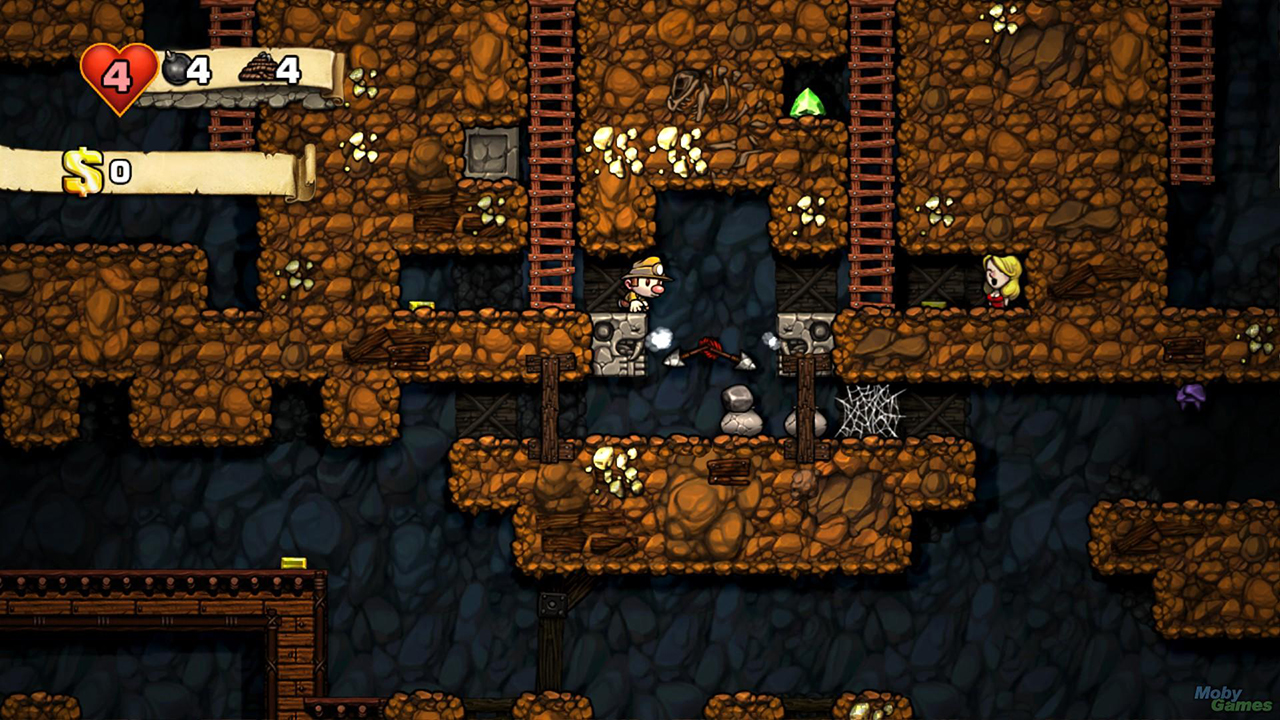
\includegraphics[width=.25\linewidth]{images/game_spelunky}
	\caption{Spelunky - Environments in Spelunky }
	\label{fig:spelunky}
\end{figure}}
\item[Positives]{
\begin{itemize}
\item{Although it is very difficult, the difficulty rarely feels unfair. Players usually feel responsible for their own deaths and, having learned from their mistakes, will be motivated to try again rather than get frustrated at the mechanics.}
\item{As a player gets more skilled, they are able to progress further into the game. The enemies become more aggressive and use more complex patterns in later areas, providing extra challenge for advanced players.}
\item{There is a soft time limit which makes levels more difficult if a player lingers for too long. This makes gameplay more exciting by forcing players to keep moving, and highly skilled players can use the time limit to their advantage to gain extra resources.}
\item{Since the random elements of Spelunky are deterministic, the developers included a mode which allows everyone to play the same seed once a day in order to compete on even ground.}
\end{itemize}
}
\item[Negatives]{
\begin{itemize}
\item{Even with an in-game tutorial with visual guides, new players struggle with the relative complexity of the controls.}
\item{The tutorial will not let you progress without completing certain lessons, but compresses multiple mechanics into single lessons, making them too challenging for new players.}
\end{itemize}
}
\item[Take-away]{The in-game tutorial for \ourgame{} must be very sequential. Attempting to communicate too many new concepts with a single task can cause players to be overwhelmed.

As \ourgame{} makes heavy use of procedural generation, ensuring that the random elements are all deterministic would allow \ourteam{} to take advantage of seed-sharing in order to create experiences such as Spelunky's daily challenge.}
\end{description}



\clearpage
\subsection{Space Channel 5 Part 2}
\begin{description}
\item[Description]{Space Channel 5 puts the player in control of Ulala, a space reporter who works to save the galaxy from evil, mostly through dancing in space. The game is rhythm-based, and is essentially an incredibly elaborate version of "Simon Says".

\begin{figure}[htb]
	\centering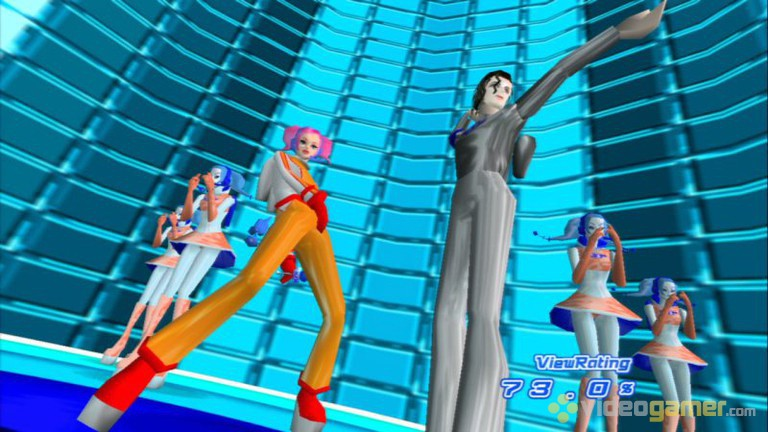
\includegraphics[width=.25\linewidth]{images/game_sc5}
	\caption{Space Channel 5 Part 2 - The game is known for its choreography and the inclusion of Space Michael Jackson as one of the supporting characters}
	\label{fig:space_channel_five}
\end{figure}}
\item[Positives]{
\begin{itemize}
\item{Players receive audio-visual feedback so that they can clearly see and hear the results of each button press in a sequence. This feedback is usually relative to the context of the scene, which can help a player to infer which buttons to press if they forgot the sequence.}
\item{The game introduces the controls in their entirety during the tutorial sequence, and difficulty is increased by re-using the same controls in progressively more complex sequences. This prevents the player from feeling blind-sided or frustrated by a sudden control change.}
\item{In-between the main gameplay sections, the player may discover secrets in order to increase their chances of winning a given level. This encourages repeated playthroughs of completed levels.}
\end{itemize}
}
\item[Negatives]{
\begin{itemize}
\item{Although some players appreciate the overall level of camp and cheesiness, this aspect can also turn away many players.}
\item{The game had noticeable issues with responsiveness. As the gameplay is rhythm-based, a minor lag between player input and the outcome in-game severely damages the player's ability to keep up with the fast-paced gameplay.}
\item{The repetition mechanic initially relies heavily on audio, letting the player listen to and understand each step of the dance sequences. Unfortunately, certain characters do not speak clear enough, creating artificial difficulty barriers and unintentional difficulty spikes.}
\item{Making a mistake costs the player a health unit and also reduces the available health during a boss fight. This often causes player frustration, as they are punished twice for a single mistake.}
\item{There are limited checkpoints within each level, and the checkpoints save the player's health when they are hit. This often leads to players getting stuck at a checkpoint after making multiple mistakes, forcing them to restart entire levels.}
\end{itemize}
}
\item[Take-away]{\ourgame{} similarly takes place in a very strange world full of unusual characters. \ourteam{} will have to take care that the eccentricity of the design does not make too many players uncomfortable, and remains an enjoyable experience.

The yelling contest mechanic in \ourgame{} is also rhythm-based. With this in mind, \ourteam{} hopes to avoid many of the issues with Space Channel 5's progression, while incorporating the well-designed core mechanic.}
\end{description}


\clearpage
\subsection{Icepunk}
\begin{description}
\item[Description]{Icepunk is a piece of interactive fiction developed in Twine and represented with text and ASCII artwork. The player in Icepunk is tasked with collecting data in a post-apocalyptic world. This data is represented in the form of short, random events that the player comes across, many of which are pulled from a database of other works of fiction released into the public domain.

\begin{figure}[htb]
	\centering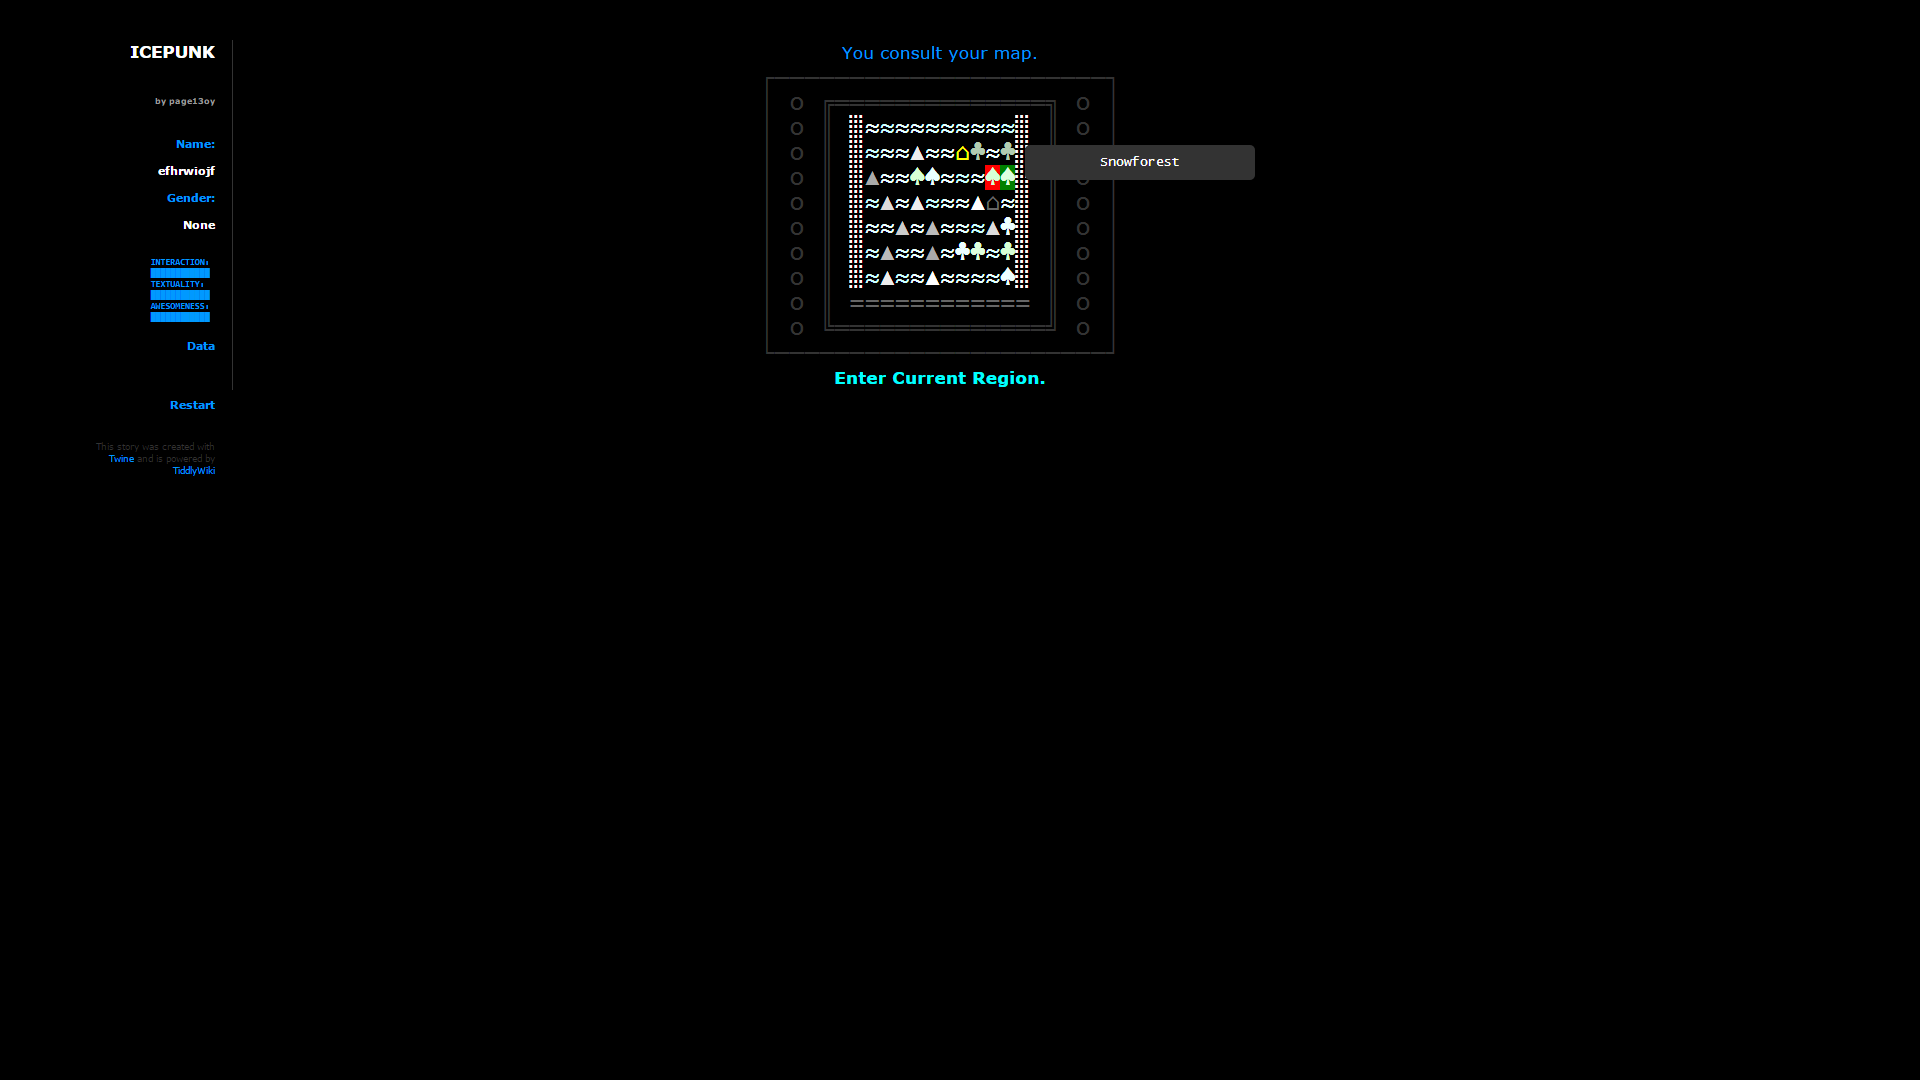
\includegraphics[width=.25\linewidth]{images/game_icepunk}
	\caption{Icepunk - Navigating the game world}
	\label{fig:icepunk}
\end{figure}
}

\item[Positives]{
\begin{itemize}
\item{Of the random events that occur throughout the game, \ourteam{} found the ones which had been written by the game's author to be interesting.}
\end{itemize}}

\item[Negatives]{
\begin{itemize}
\item{The length of text given for many segments was sometimes intimidating.}
\item{The UI, specifically for navigation, left much to be desired. The player could only move one unit at a time, causing it to take too long to get from point A to point B. Some players were also confused by the inability to move anywhere on the map, causing them to highlight other areas accidentally, resulting in visual feedback that didn't actually affect the game state.}
\item{The game's primary mechanics were exploration and collection of resources, but the limited inventory discouraged players from traveling too far from the home base.}
\item{The repetitiveness of the gameplay combined with the lack of variety made most players give up early on in the experience.}
\end{itemize}}

\item[Take-away]{\ourteam{} did not enjoy Icepunk. There were tidbits of interesting design, but the feeling that most of the game was going to be a slog of repetitive gameplay and random public domain excerpts made it all feel meaningless. By playing this game, \ourteam{} resolved to produce a large number of story elements to reduce repetition, and to ensure the text is broken up by different audio-visual elements so as not to overwhelm players with large amounts of text.}
\end{description}



\clearpage
\subsection{Sunset}
\begin{description}
\item[Description:]{Sunset is an atmospheric game which puts the player in the shoes of a US citizen stuck in a small Latin American country in the middle of a military coup. The player is tasked with housekeeping for a wealthy individual, and over the course of the game can become involved in the political plots taking place. The game was a commercial failure.

\begin{figure}[htb]
	\centering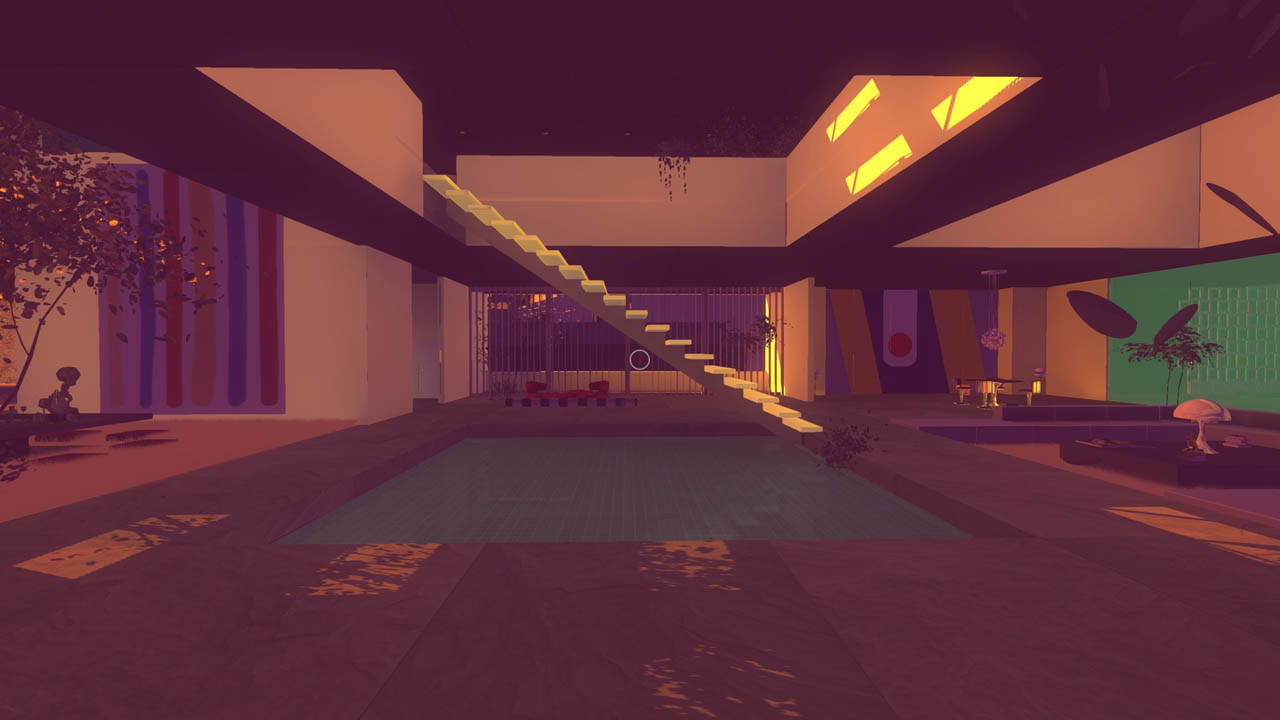
\includegraphics[width=.25\linewidth]{images/game_sunset}
	\caption{Sunset - The apartment which serves as the gameplay area}
	\label{fig:sunset}
\end{figure}}

\item[Positives]{
\begin{itemize}
\item{Visual design and lighting was very nice.}
\end{itemize}}

\item[Negatives]{
\begin{itemize}
\item{The player character representation was very lackluster. The animation was very basic and put the character into the uncanny valley.}
\item{The camera placement was disproportional to the game's environment, and resulted in the player feeling like they were a giant in a house for tiny people.}
\item{The menus and instructions were an overwhelming mish-mash of complicated controls presented to the player all at once when the game is started.}
\item{After interacting with objects, the player would sometimes be transported to other areas of the house without any indication of what had happened.}
\end{itemize}}

\item[Take-away]{Overall, the game reminded \ourteam{} of other, similar games such as Gone Home or Dear Esther, but did not seem to bring anything new to the table. Some members hypothesized that the game was a failure, not because it was uninteresting, but because the first impressions made by the terrible in-game menus and initial tutorial negatively affected most players' opinions of the game as a whole.}
\end{description}



\clearpage
\subsection{Rogue Legacy}
\begin{description}
\item[Description]{Rogue Legacy is a rogue-"lite" in which the player takes control of a single family's lineage, sending descendant after descendant into the depths of a castle in order to retrieve the treasures inside. The idea of carrying the family towards victory over the generations plays into the gameplay heavily.

\begin{figure}[htb]
	\centering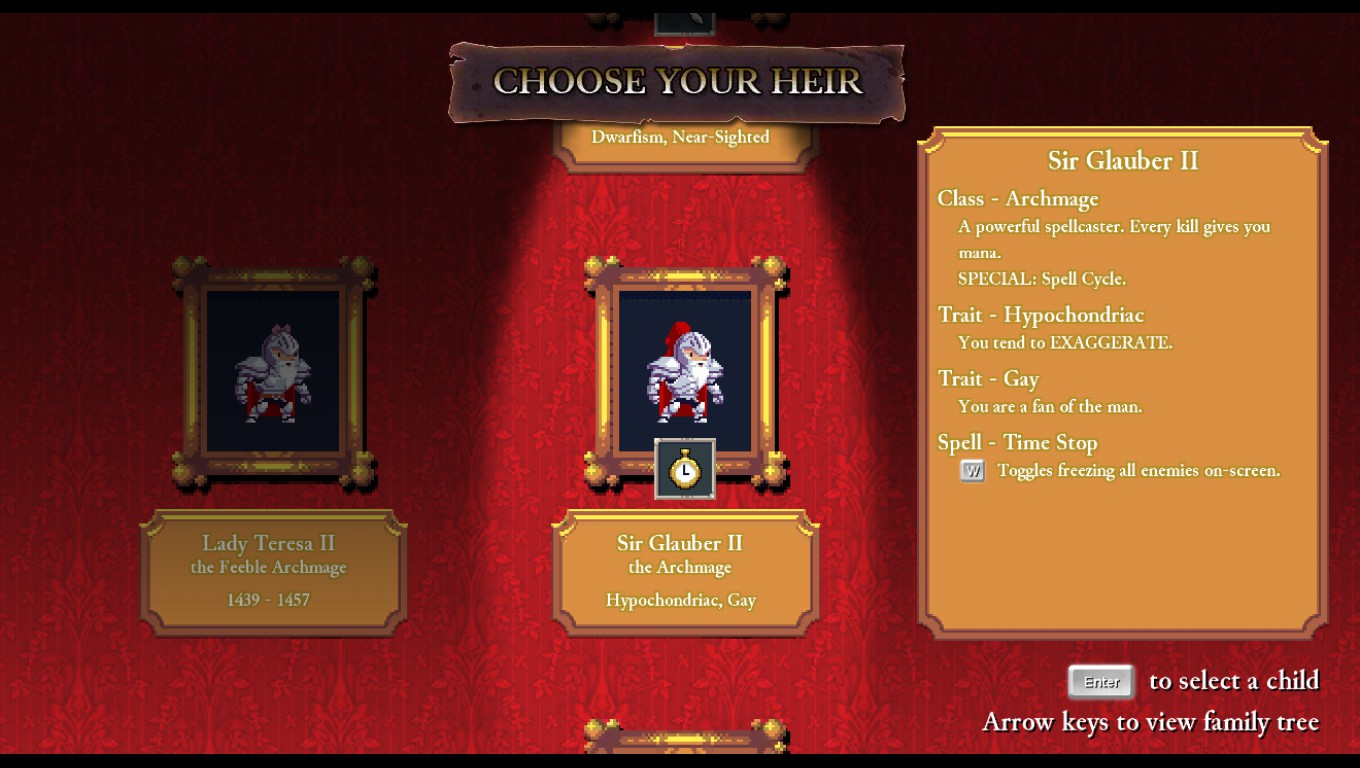
\includegraphics[width=.25\linewidth]{images/game_rogue_legacy}
	\caption{Rogue Legacy - The character selection screen, which shows the lineage from the player's first character to their last}
	\label{fig:rogue_legacy}
\end{figure}}

\item[Positives]{
\begin{itemize}
\item{Effective use of pixel art.}
\item{The procedurally generated characters and traits give each run a unique feel. This is enhanced by letting the player choose between three characters, making them feel more responsible for the run's outcome.}
\item{Once defeated, bosses remain dead until the game is completed. This helps the player to feel they are making progress even if they cannot beat multiple bosses in a single run.}
\end{itemize}
}
\item[Negatives]{
\begin{itemize}
\item{The game's difficulty is largely based on mechanical player progression; the player is rewarded more for simply spending time playing the game than they are for actually learning how to play it properly. This can make extended gameplay feel like grinding, and make more difficult enemies seem unfair at earlier stages in the game.}
\end{itemize}
}
\item[Take-away]{The idea that the progress made by the player is preserved, regardless of the fact that they are playing multiple runs of the same game is reflected in the progression of \ourgame{}'s plotline.}
\end{description}



\clearpage
\subsubsection{Runescape Classic}
\begin{description}
\item[Description]{Runescape is a browser-based MMORPG that takes place in a standard fantasy setting. The game is primarily known for presenting players with an expansive game world with a variety of activities and quests in the early ages of online gaming.

\begin{figure}[H]
	\centering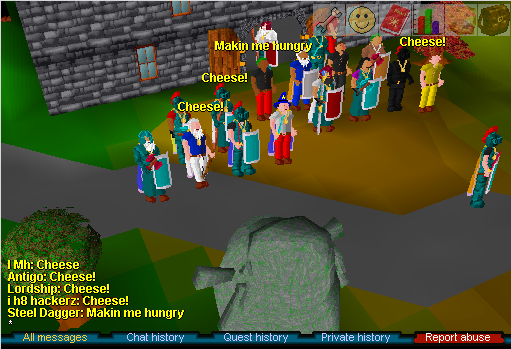
\includegraphics[width=.25\linewidth]{images/game_runescape}
	\caption{Runescape - Player interacting with other players}
	\label{fig:runescape}
\end{figure}
}
\item[Positives]{
\begin{itemize}
    \item{Quest system is exploration based, providing the player with freedom to explore the world while completing quests.}
    \item{Social interactions between players in the online environment can improve the experience.}
    \item{The great soundtrack enhances the experience.}
\end{itemize}
}

\item[Negatives]{
\begin{itemize}
	\item{The gameplay and visuals are very outdated by modern standards.}
    \item{There is an in-game tutorial to help new users, but it is far too long and can easily turn away those eager to start playing.}
    \item{The controls are not streamlined, resulting in tedious gameplay.}
    \item{The UI is outdated and complicated, making heavy use of nearly illegible text. Players may have difficulty finding and reading crucial information, preventing them from playing the game effectively.}
    \item{As an MMO, it requires a big social component, but there are very few features which highlight interaction with other players. Player-player interaction is limited to chat, trading, and a specific player-versus-player combat zone.}
    \item{Many of the quests are specifically designed to take advantage of the player's limited inventory by forcing them to make multiple trips to collect items.}
\end{itemize}
}
\item[Take-away]{Runescape places the player in a vast, complex world capable of capturing the player's interest with interesting characters and variety of quests. Aside from this, \ourteam{} found Runescape to be largely uninteresting. The unusable UI, outdated graphics/gameplay, and poorly constructed systems make the game difficult to play. It is obvious that a strong effort must be put into polishing user facing systems in \ourgame{}. Additionally, although the social component certainly improves Runescape, the potential for improvement in \ourgame{} is fairly limited and including other players in a narrative experience could easily detract from the immersive environment and lore \ourteam{} intends to create.}
\end{description} 